\begin{figure*}[ht]
\centerline{
    \includegraphics[width=\textwidth]{images/plot_DSE_6RoI_2.jpg}
    }
    \caption{Pareto-plot for simulation - \gls{qoc} vs given platform allocation, i.e., $\numCoresAvailable$. Here, we consider the \gls{sadf} in Fig.~\ref{fig:ch7_SADF}~(a) with $z=6$ (worst-case workload). The \gls{mse} and \gls{st} are normalised with respect to the maximum (worst-case) value. The legend denotes $<\numCoresAvailable,\ \numCoresParallel,\ \numPipes>$. Higher \gls{gm} and \gls{pm}, and lower \gls{mse} and \gls{st} are better.}
    \label{fig:ch7_Pareto}
    \vspace{-1em}
\end{figure*}

\section{Experimental results and discussion}
\label{sec:ch7_ExperimentalResults}
This section explores the \gls{spade} experimental results with a focus on \gls{dse}.
The \gls{dse} is used for identifying the degrees of parallelism and pipelining for the pipelined parallelism implementation.
A \gls{dse} is required since the parallelisation is limited by the degree of application parallelism quantified using $\numCoresParallel$ and $\numCoresAvailable$, and the maximum number of active pipes we can have is limited by $\fd$, $\fh$, $\numCoresParallel$ and $\numCoresAvailable$.
After exploring the \gls{dse} results for the running example, we discuss a few observations for the \gls{spade} flow and compare the state-of-the-art methods with our proposed \gls{spade} flow for pipelined parallelism. The simulations in this section consider the \gls{lkas} case study introduced in Section~\ref{sec:lkas_case_Study}. The \gls{lkas} is modelled using the \gls{ibc} graph given in Fig.~\ref{fig:ch7_SADF}~(a) with the worst-case workload scenario having $z=6$ and the execution times of the actors as explained in Section~\ref{sec:ch7_IBCGraph}. The platform we consider is the predictable \gls{compsoc} platform (as explained in Section~\ref{sec:compsoc}) with $\numCoresAvailable$ as an input to the \gls{spade} flow.

\subsection{\texorpdfstring{\Acrfull{dse}}{Design space exploration (DSE)}}
\label{sec:ch7_DSE}
The \gls{spade} flow has been explored till now with a fixed number of pipes $\numPipes$ and a fixed number of cores per pipe for parallelism $\numCoresParallel$.
A \gls{dse} with design parameters $\fh,\ \numPipes,\ \numCoresParallel,\ \numCoresAvailable$ is needed to identify the Pareto-optimal implementation choice, i.e., the degree of pipelining and the degree of parallelism.
Note that $\numPipes$ quantifies the degree of pipelining, and $\numCoresParallel$ quantifies the degree of application parallelism for an implementation choice.
Typically, $\fh$ and $\numCoresAvailable$ are given or fixed. We only vary these two parameters if the goal is to identify the optimal frame rate or minimise resource usage.

We use a brute force method to identify the possible implementation choices $<\numCoresAvailable,\ \numCoresParallel, \numPipes>$ over the design space. For each implementation choice, i.e., with fixed design parameters, we compute its \gls{gm} and \gls{pm} (see Section~\ref{sec:ch7_QoC_metrics}) for the worst-case system scenario $s_{s_{wc}}$ (see Step~\ref{algoStep:tau_swc_h_s_wc} in Algorithm~\ref{algo:SPADeFlow}).
\gls{gm} and \gls{pm} are analytical metrics and can be computed easily from the discretized control system model in Eq.~\ref{eq:ch7_cld2} for $s_{s_{wc}}$.
We suggest using \gls{gm} and \gls{pm} to prune the design space to be explored for multiple implementation choices, as the \gls{mse} and \gls{st} \gls{qoc} metrics that we ultimately want to optimise are simulation-based and obtaining them is compute-intensive.
A performance comparison for different implementation choices using \gls{mse} and \gls{st} is moreover unfair unless we can do exhaustive simulation considering different initial conditions and environments (e.g., weather conditions, as illustrated in our previous work~\cite{de2020access}).

Thus, the Pareto-optimal implementation choice for a given platform allocation $\numCoresAvailable$ is chosen as the one with the highest \gls{gm} and \gls{pm}.
If \gls{gm} and \gls{pm} are incomparable for multiple implementation choices for a platform allocation, in the sense that one implementation choice has a higher \gls{gm} and the other one a higher \gls{pm}, then we consider both these choices as part of the Pareto front. The Pareto-optimal implementation choices are further analysed using \gls{mse} and \gls{st}.
To do so, controllers are designed for the Pareto-optimal implementation choices, and optimal system scenarios considering workload variations are identified based on control performance metrics \gls{mse} and \gls{st}.

As a proof-of-concept, we performed \gls{dse} with $\fh=\frac{1}{60}$ and given (maximum) platform allocation of six processing cores, i.e., $\numCoresAvailable=6$, considering the \gls{ibc} graph in Fig.~\ref{fig:ch7_SADF}~(a).
The \gls{qoc} over various design points is illustrated in Fig.~\ref{fig:ch7_Pareto}. For the purpose of validation, we explored more implementation choices through simulation than only the Pareto-optimal ones as described above.
The results show that the implementation choices with higher gain and phase margins indeed have better control performance (\gls{mse} and \gls{st}) in the simulations, confirming that \gls{gm} and \gls{pm} can be used to prune the design space. 
The only anomaly is the normalised \gls{st} for the case $<2,2,1>$ for two cores which is better than the \gls{st} for the configurations with a higher number of cores. 
We observe that this is due to our simulations proceeding at the rate of the sampling period. E.g., the sampling period for both the cases $<2,2,1>$ and $<3,3,1>$ is the same (0.0667~ms), but their sensor-to-actuator delays are 0.065~ms and 0.055~ms, respectively. When we proceed with the simulations at the rate of the sampling period, the slight differences in the settling time are due to approximations in the model fitting. 

In terms of optimising \gls{qoc} for the running \gls{lkas} example, an important first observation from the \gls{dse} results is that all configurations that exploit parallelism and/or pipelining improve \gls{qoc} over the fully sequential implementation $<1,1,1>$.
Our simulations moreover show that, typically, for the optimal \gls{qoc}, we should parallelise as much as possible (increasing $\numCoresParallel$) and then pipeline (increasing $\numPipes$).
For example, in Fig.~\ref{fig:ch7_Pareto}, let us consider the cases of $\numCoresAvailable=3$ and $\numCoresAvailable=6$.
Among the configurations with $\numCoresAvailable=3$, we notice that the configuration $<3,3,1>$ has the highest \gls{gm} and \gls{pm} and the best control performance. 
The normalised \gls{mse} is similar for both $<3,3,1>$ and $<3,1,3>$. There is a visible improvement in the normalised \gls{st} for the first of these two configurations that maximises parallelism compared to the second that maximises pipelining.
Similarly, when $\numCoresAvailable=6$, we notice that configuration $<6,6,1>$ has the highest \gls{gm} and \gls{pm} and best normalised settling time. 
The normalised \gls{mse} is similar to the cases $<6,3,2>$ and $<6,2,3>$. We observe that this is due to having the same sampling period for all these cases. 
The trend that parallelisation should be prioritised over pipelining is true for other platform allocations.

Let us now consider the cases of $\numCoresAvailable=4$ and $\numCoresAvailable=5$.
It is interesting to notice that the control performance for both these cases is identical, and the performance does not improve by allocating one more core when $\numCoresAvailable=4$.
This is due to identical control timing parameters, delay and period, when $\numCoresAvailable=4$ and $\numCoresAvailable=5$.
It is also interesting to note that the fully parallelisable implementations $<4,4,1>$ and $<5,5,1>$ do not have the best performance for both these cases. 
This is because of identical delay (= 55~ms) and period (= 66.7~ms) when $\numCoresParallel=\numCoresAvailable$ and $p=1$, for the cases with $\numCoresAvailable={3,4,5}$.
This happens because when we distribute six \glspl{roi} over 3, 4 or 5 cores, there are always two sequential \gls{roi} executions needed on (at least) one core, meaning that the effective delay does not change. 
This means that we already have a fully parallelisable implementation with $\numCoresAvailable=3$. 
When we have a fully parallelisable implementation and still have more cores available, we can pipeline.
E.g., the cases with the best performance for $\numCoresAvailable={4,5}$ are $<4,2,2>$ and $<5,2,2>$. These cases have delay and period equal to 65~ms and 33.3~ms, respectively. 
We observe that considering parallelism and pipelining integrally has better performance than considering only one of the two options.

The main conclusion of the \gls{dse} is that we should \textit{parallelise as much as possible and then pipeline while taking into account the delay and period}. 
It is important to note that increasing the number of available cores does not necessarily improve the control performance. This is due to several factors. The most prominent factors, the camera frame rate and the inter-frame dependencies, have been discussed earlier.
Our results also show the significance of \gls{gm} and \gls{pm} in pruning the design space for exploration.
A higher \gls{gm} and \gls{pm} typically imply a better control performance (\gls{mse} and \gls{st}).
The \gls{gm} and \gls{pm} are computed analytically, whereas the \gls{mse} and \gls{st} can only be computed through simulations.
For \gls{spade}, we use this knowledge to prune the design space.

\subsection{Is higher frame rate always better?}
%\label{sec:ch7_results_fh}
Our observation with respect to the frame rate is that having a higher frame rate is not always better. 
Having a higher frame rate means processing the arriving frames at a higher rate, which is compute-intensive, and may not always improve the control performance (as shown in Fig.~\ref{fig:ch7_coresVSfhNP}). 
We observe that the control performance is similar for 60 fps and 120 fps for all the cases.
The control performance is the worst for 30 fps when we have only one available processing core.
A slight degradation in control performance is noticed for 30 fps when considering 2-5 available processing cores. 
If we have six available processing cores, all the frame rates have similar performance.
The control performance is dependent mainly on the $\tau_s$ and $h_s$ of the system scenarios.
If improving the frame rate does not effectively decrease the average delay and/or period, it becomes an overhead to do so and wastes compute resources in the given platform.

\begin{figure}[ht]
  \centering
  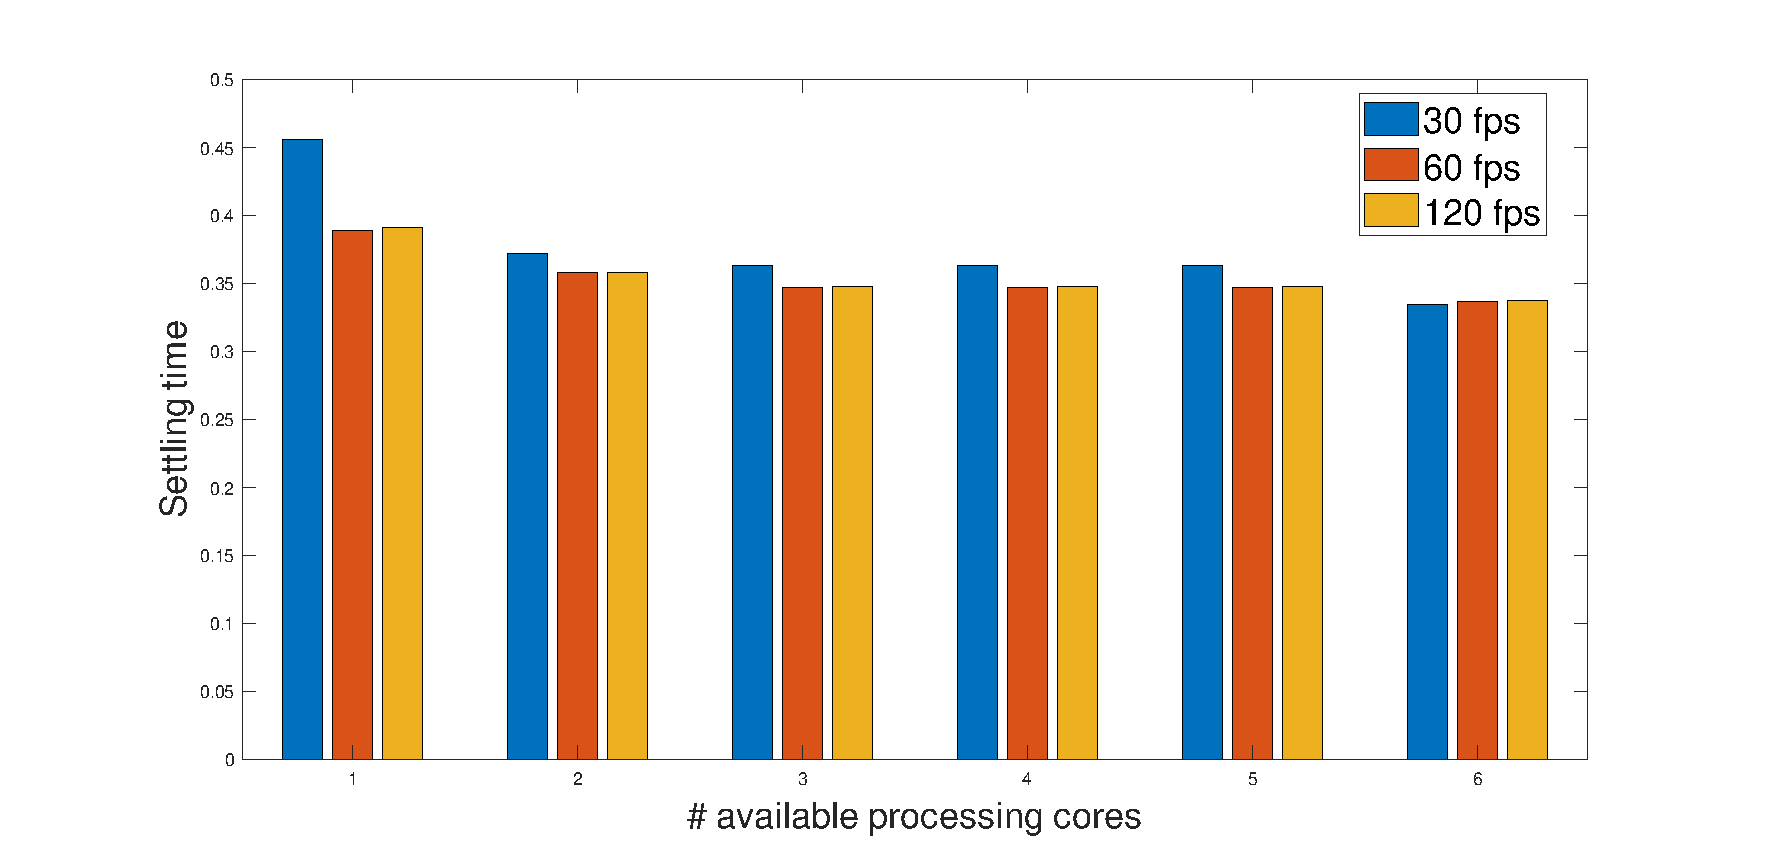
\includegraphics[width=0.8\linewidth]{images/coresVSfh.eps}   
  \caption{$\numCoresAvailable$ vs settling time (in s) considering different frame rates for the \gls{sadf} in Fig.~\ref{fig:ch7_SADF}~(a) with $\rateY=6$ (workload) and $\numPipes=1$.}
  \label{fig:ch7_coresVSfhNP}
  \vspace{-2em}
\end{figure}

\subsection{Impact of inter-frame dependencies}
%\label{sec:ch7_results_ifd}
In a pipelined implementation, the inter-frame dependencies have a significant impact on the maximum number of pipes we can realise $p_s$ (see Step \ref{algoStep:ps} of Algorithm \ref{algo:SPADeFlow}).
The impact of the inter-frame dependence time $\fd$ on $p_s$ is illustrated in Fig.~\ref{fig:ch7_fd_vs_ps} using an example. 
In this example, we allocate sufficiently many cores $\numCoresAvailable=12$ since $n_{c_{max}}=12$ (see Step~\ref{algoStep:ncmax} in Algorithm~\ref{algo:SPADeFlow}) for a camera frame rate of 120~fps, considering a worst-case delay of $\tau_{wc}=95$~ms, and $\numCoresParallel=1$. 

If $\fd=0$, the maximum number of realisable pipes we can have when the camera frame rates are 30, 60 or 120~fps are 3, 6 or 12, respectively.
E.g., if the camera frame rate is 120~fps, then we can have a maximum of $\ceil{\tau_{wc}/\fh}=\ceil{0.095\times 120}=12$ pipes.
Note that, as $\fd$ increases, the number of realisable pipes reduces exponentially.
E.g., if $\fh < \fd \le 2\fh$, then the number of frames to skip after processing each camera frame is one. Now for the camera frame of 120 fps, skipping one frame after every frame processing means that the realisable number of pipes will become 6 (see the interval $\fd=(0.0083,0.01667]$ in Fig.~\ref{fig:ch7_fd_vs_ps}).
A higher $\fd$ implies a smaller number of realisable pipes. 
Also, as $\fd$ increases beyond a certain point, pipelining is no longer feasible (when $p_s=1$). 
E.g., in Fig.~\ref{fig:ch7_fd_vs_ps}, $p_s=1$ in the intervals $\fd=(0.067,0.100]$ for 30~fps, $\fd=(0.083,0.100]$ for 60~fps, and $\fd=(0.092,0.100]$ for 120~fps.

\begin{figure}[ht]
\centerline{
    \includegraphics[width=0.8\textwidth]{images/fd_vs_ps2.jpg}
    }
    \caption{Impact of $\fd$ on maximum number of realisable pipes $p_s$. In this example, we consider $\tau_{wc}=95$~ms, $\numCoresParallel=1$ and $\numCoresAvailable=12$.}
    \label{fig:ch7_fd_vs_ps}
    \vspace{-2em}
\end{figure}

\subsection{Impact of system-scenario switching on control performance}
It is possible for switching to degrade the control performance compared to the periodic worst-case-based design (presented in Fig.~\ref{fig:ch7_Pareto}). However, we choose system scenarios such that the control performance improves even if we have switching at runtime. Further, we discard the combinations of aggregated workload scenarios that degrade control performance compared to the single worst-case workload scenario $s_{wc}$ during system-scenario identification (see Section~\ref{sec:ch7_sysConfigStability}).
We illustrate this observation using Fig.~\ref{fig:ch7_workloadVSfps} where we consider the \gls{sadf} in Fig.~\ref{fig:ch7_SADF} having three system scenarios $s_1$, $s_2$ and $s_{wc}$ with 1, 3 and 6 \gls{roi} respectively. $s_1$ is the best-case workload scenario with the smallest delay and $s_{wc}$ is the worst-case scenario with the worst-case delay.
Notice that, in all switching cases, the control performance settles faster than the periodic worst-case based design (denoted by $(s_{wc})^\omega$ in Fig.~\ref{fig:ch7_workloadVSfps}).
The trend is similar for different camera frame rates as well.
We observe that the control performance is better if the frequently occurring workload scenario is closer to the best case than the worst case. E.g., in Fig.~\ref{fig:ch7_workloadVSfps}, the scenario sequence $(s_1^{10}s_{wc})^\omega$ has $s_1$ as the frequently occurring scenario, which leads to a better performance than $(s_2^{10}s_{wc})^\omega$ with $s_2$ as the most frequently occurring scenario.
Further, we observe that the control performance of the scenario sequences cluster towards the performance of its most frequently occurring scenario, as is observed in Fig.~\ref{fig:ch7_workloadVSfps} with distinct colour regions (where the blue and green scenarios form one cluster).

\begin{figure}[t]
  \centering
  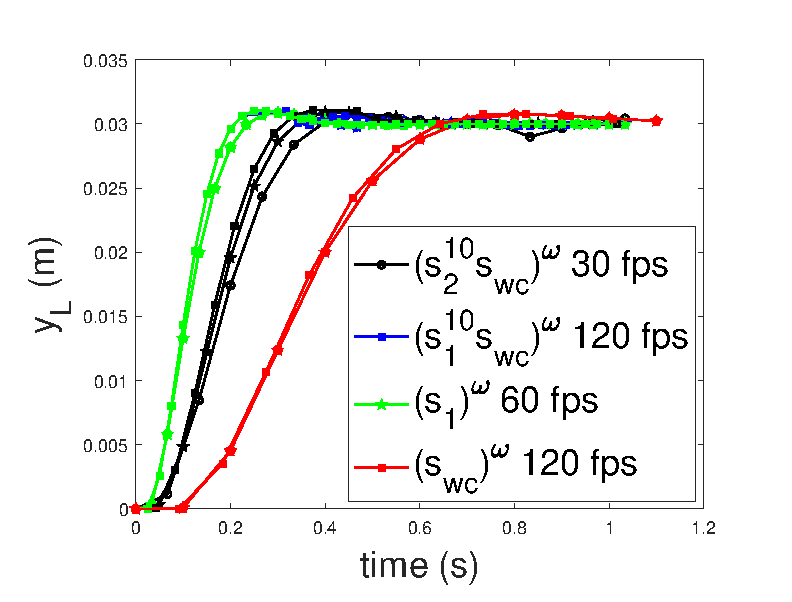
\includegraphics[width=0.7\textwidth]{images/workloadVSfps.eps}  
  \caption{Impact of system scenarios switching due to workload variations on $y_L$ with $\numCoresAvailable=1$. Note that the legends mention representative scenario sequences; the plot contains more scenario sequences than the ones mentioned in the legends. The markers denote the frame rate and colours denote the scenario sequences.}
		\label{fig:ch7_workloadVSfps}
\end{figure}

\begin{table*}[t]
\centering
\caption{Comparing the proposed \gls{spade} approach with the state-of-the-art multiprocessor \gls{ibc} system implementations}
\label{tab:ch7_my-table}
\resizebox{\textwidth}{!}{%
\begin{threeparttable}	
\begin{tabular}{|p{2.9cm}|p{3.9cm}|p{2.9cm}|p{2.5cm}|p{2.9cm}|}
\hline
\multicolumn{1}{|c|}{\multirow{2}{*}{Criteria}} &
  \multicolumn{1}{c|}{\multirow{2}{*}{\Gls{spade} approach}} &
  \multicolumn{2}{c|}{Pipelined} &
  \multirow{2}{*}{Chapter \ref{chap:parallelisation}} \\ \cline{3-4}
\multicolumn{1}{|c|}{} &
  \multicolumn{1}{c|}{} &
  \multicolumn{1}{c|}{~\cite{krautgartner1998performance},~\cite{medina2019designing},~\cite{medina2019implementation}} &
  \multicolumn{1}{c|}{Chapter \ref{chap:pipelined}} &
   \\ \hline
Inter-frame dependencies    & explicitly considered   & not considered           & considered         & independent          \\ \hline
System non-linearities & control-design dependent & not considered & explicitly considered & not considered in Chapter \ref{chap:parallelisation}; control-design dependent \\ \hline
Constraints on variables & control-design dependent & cannot be imposed & can be strictly imposed & not considered in Chapter \ref{chap:parallelisation}; control-design dependent \\ \hline
Control computation time & low & low - medium & high & low \\ \hline
Runtime overhead due to reconfiguration               & explicitly considered as a time cost in the \gls{sadf} model    & not considered \cite{krautgartner1998performance}\cite{medina2019designing}; not explicitly considered \cite{medina2019implementation} & explicitly considered   & explicitly considered \\ \hline
Algorithm                 & white/gray/black box    & white/gray/black box     & white/gray/black box   & white/gray box \\ \hline
Parallelisation potential & explicitly taken into account             & independent              & independent            & should be high       \\ \hline
Workload variations       & explicitly considered in design             & not considered \cite{krautgartner1998performance}\cite{medina2019designing}; indirectly considered \cite{medina2019implementation} & explicitly considered in design  & explicitly considered \\ \hline
Platform                  & can be adapted for all  & suitable for homogeneous \cite{krautgartner1998performance}\cite{medina2019designing}; can be adapted for all \cite{medina2019implementation} & suitable for homogeneous & directly applicable for all   \\ \hline
Resource sharing between pipes & explicitly considered during mapping & not considered & not considered & not applicable \\ \hline
Restrictions on sampling period $h$\tnote{1}      & strictly periodic for pipelined, $h < \tau_{wc}$; switched for non-pipelined;  &  strictly periodic; $h < \tau_{wc}$    &  strictly periodic; $h < \tau_{wc}$  & switching possible
\\ \hline
Restrictions on sensor-to-actuator delay $\tau$  & none   & strictly $\tau_{wc} > h$; in~\cite{medina2019designing}, $\tau$ is strictly a multiple of $h$ & strictly\tnote{2}~~ $\tau_{wc}>h$  & $\tau_{wc} \le h$   \\ \hline
\end{tabular}%
\begin{tablenotes}
			\footnotesize
			\item{$\tau_{wc}$: worst-case delay;\ $^1$ If camera frame arrival period $\fh$ is considered, always $h$ is a multiple of $\fh$; $^2$ if $\tau_{wc}\le h$ design reverts to non-pipelined.} 
		\end{tablenotes}
		\end{threeparttable}
}
%\vspace{-2em}
\end{table*}

\subsection{Comparison with the state-of-the-art}
The \gls{dse}, as explained in Section~\ref{sec:ch7_DSE} and illustrated in Fig.~\ref{fig:ch7_Pareto}, already shows quantitatively that integrally considering the combination of parallelism and pipelining in multiprocessor \gls{ibc} design outperforms the state-of-the-art approaches in which only one of the two options is considered. The integral consideration of parallelism and pipelining differentiates \gls{spade} from any earlier work, as explained in Section \ref{sec:sota}. In this subsection, we compare the proposed \gls{spade} method qualitatively on several other relevant criteria with state-of-the-art multiprocessor \gls{ibc} design techniques in Table~\ref{tab:ch7_my-table}. 
For brevity, we only compare with multiprocessor \gls{ibc} system implementations and not with traditional sequential control design techniques based on the worst-case sensing delay, as it has already been shown in Chapter \ref{chap:parallelisation} and \cite{fontantelli2013optimal} that multiprocessor implementations are beneficial for optimising control performance.
The multiprocessor implementations can be classified into pipelined~\cite{krautgartner1998performance},~\cite{medina2019designing} with constant delay, pipelined with variable delay~\cite{medina2019implementation} and pipelined with workload scenarios (Chapter \ref{chap:pipelined}), and sequential implementation with parallelisable sensing that is explained in Chapter \ref{chap:parallelisation}.
The camera frame rate, however, is not explicitly considered in~\cite{krautgartner1998performance}.

The proposed approach is advantageous to other multiprocessor \gls{ibc} system implementations with respect to: 1) coverage of the design space considering both pipelining and parallelisation; 2) considering inter-frame dependencies and resource sharing among pipes; and 3) not imposing any restrictions on $\tau$, thereby enabling shorter $\tau$ and $h$ compared to other approaches.